\documentclass[12pt]{article}
\usepackage{graphicx}
\usepackage{pstricks}
%\usepackage{pstricks-add}
%\usepackage{pst2pdf}
\usepackage{float}
\graphicspath{{./Figures/}}


\begin{document}
\section{In Read\_data.py}
We begin by reading \texttt{travel\_times\_2011.csv} using csv.DictReader. 
Using \\\textsl{read\_data\_csv}, we then save the trips and travel times data in sparse coordinate matrix form, i.e. (hour (in EDT), link, trips, traveltimes), as \texttt{data\_coo\_form.txt}. 
Next, using \textsl{write\_data\_array},  we write these values to \texttt{data\_trips.csv} and \texttt{data\_travel\_times.csv}. 
For an unknown reason, \textsl{write\_data\_array} introduced a line break in the first hour of the first day of data.
After correcting this break, we reverse the order of the data from the previous step since the data is given in descending order, but we need to write it in ascending order.
This is fairly memory intensive due to the scale of the data so we utilized the campus cluster for efficiency. 

Next, we want to pull out the data corresponding to links with at most 30 days worth of data missing; this is done with \textsl{find\_full\_links}. 
We also ran this on the campus cluster.
The list of full link ids is saved under \texttt{full\_link\_ids.csv}.
We then pull the corresponding data for these links using write\_full\_link\_data and save into \texttt{write\_full\_link\_trips.csv} and \texttt{write\_full\_link\_traveltimes.csv}.
Henceforth, \textsl{read\_full\_link\_json} should be used to return the full link ids and their data.

Then, we want to find the periodicity of the full link data. 
By running autocorrelation, we see that the period is 7 days. 
We check the refinement of this by running autocorrelation\_hourly, and verify the 7-day period.
We also checked the periodicity of the travel times and it matches the 7-day period (graph omitted but is saved in Figures\textbackslash).

\begin{figure}[H]
\centering
\includegraphics[width=.9\textwidth]{Autocorrelation_Full_Links.ps}
\end{figure}

\begin{figure}[H]
\centering
\includegraphics[width=.9\textwidth]{Autocorrelation_Full_Links_hourly.ps}
\end{figure}

\section{In Phase1.py}
% Beware NaN is a float so int(NaN) returns error
We group the functions for running Sparse Non-negative Matrix Factorization under \textsl{find\_signatures}.
Using the campus cluster, we run SNMF with $\beta$, $\eta$, and rank ?????
Running SNMF(traveltimes, rank=50, $\beta=0.1$, $\eta=0.1$, threshold=$0.01$) gives error of 39.890\%. 
Running SNMF(trips, rank=50, $\beta=0.1$, $\eta=0.1$, threshold=$0.01$) gives error of 28.666\%. 

\end{document}
